% !Mode:: "TeX:UTF-8"
\chapter{绪论}
\label{cha:intro}

本章首先介绍了基于大模型智能问答系统的选题背景及研究意义,接着介绍了大模型表格数据推理及RAG问答系统的国内外研究现状,通过国内外相关研究进展引出了本文的主要研究内容及工作要点,为后续章节主要研究工作的论述做好铺垫,最后介绍了论文的结构。
 
\section{课题研究的目的和意义}
检索增强生成(Retrieval-Augmented Generation, RAG)技术,实现了从外部知识库中检索相关信息并将其作为上下文输入到大语言模型中,从而生成更准确、更相关的答案。该系统主要包含两个阶段:首先,使用检索模型根据用户问题检索相关文档;然后,以检索到的上下文为基础,利用大语言模型生成最终的回答。

近年来,大模型问答系统和大模型表格推理技术在金融分析、社会服务和专家咨询等垂直领域加速落地,推动了人工智能在智能交互与信息处理领域的应用,助力国家数字经济和智能化发展的战略目标。该方向的研究紧密结合中国“数字中国”建设和《新一代人工智能发展规划》的建设需求,具有重要的理论与实践价值。通过研究大模型问答系统,可提升自然语言理解和生成技术在政务、医疗、金融等领域的实际应用能力,提高信息交互效率;而大模型表格推理技术则能实现对结构化数据的自动解析与推断,为复杂的决策支持、数据分析和业务管理提供高效和精准的技术解决方案。

在大模型问答系统推理及部署相关技术中,由于推理框架中的各种模型参数较大,需要较高的存储和运算能力,而对于实时提供问题回答的问答系统,推理速度显得尤为重要。所以,模型的轻量化压缩技术是提高模型响应速度,改善用户体验的关键技术。大模型的问答系统在如金融、医疗和科研等众多领域有广泛的应用\cite{1024008988.nh,1024532352.nh,1024651093.nh,1024744443.nh,1024917032.nh},针对问答系统的开发,确定的应用场景极为关键。

在常微分方程神经网络(Ordinary Differential Equation Neural Network)\cite{chen2018neural}的提出下,动力学系统微分方程和神经网络的结合进入大众视野。研究者逐渐将神经网络与动力学系统相联系,利用动力学系统中成熟且丰富的方法处理神经网络模型。借助动力学系统模型降阶的方法应用于神经网络的模型压缩中,能够提出新的模型压缩方法并验证两个领域存在联系,提高神经网络模型的理论可解释性,并为后续神经网络的理论研究提供思路。同时在大模型的嵌入层应用压缩算法,提高模型的推理速度,进而提高智能问答系统的相应速度。

大模型问答系统的开发离不实际工程应用场景。开发完整的问答系统需要成熟的向量数据库存储及检索技术及框架,大模型检索增强推理技术应用部署框架及网络部署框架,来提高基于本地知识库的高并发性、可扩展性和高响应速度。为提高大模型的表格数据推理能力,还需要额外引入Agent代理思想,运用数据库技术提升对数据的处理能力。来满足针对特殊场景下不同结构文本数据的理解能力,有效解决面对表格数据问题的幻觉问题从而提高回答质量。

基于以上背景及目的意义,本文研究了基于本征正交分解的循环神经网络模型压缩算法和大模型表格数据推理框架,设计了面向水利水库调度领域的基于本地知识库的大模型智能问答系统,最后完成了知识库及其大模型问答系统的落地部署。



\section{国内外研究概况}
\subsection{RAG系统研究概况}
LLM(Large Language Model,大语言模型)\cite{he2024annollm,weifinetuned,chen2023label,chung2024scaling,longpre2023flan}的出现为NLP(Nature Language Process,自然语言处理)领域任务带来了巨大改变与提升。OpenAI在2020年和2023年发布的GPT类大模型\cite{floridi2020gpt},以及2023年发布的Llama\cite{touvron2023llama}系列大模型和Gemini\cite{team2023gemini}等大模型在多项NLP任务中都达到了前所未有的高度。甚至在一些任务中的表现超过了人类\cite{lu2018beyond,hendrycksmeasuring}。
尽管大语言模型在许多任务中都展现了强大的能力,但其仍存在一些需要改进的地方。例如,在面对复杂问题或特定领域时,模型可能生成不准确的信息\cite{zhang2023large}。当用户的查询超出模型训练数据范围,或者需要最新信息时,模型的知识储备可能显得不足 \cite{kandpal2023large}。这种局限性在生成式人工智能的实际应用中尤为突出,仅依赖于不透明的大语言模型通常无法满足生产环境的要求。虽然通过微调可以使传统神经网络适应特定领域,但这种方法需要大量计算资源和专业技术,且在动态更新的信息环境中适应性较差。

大语言模型的知识储备主要分为参数化知识和非参数化知识。参数化知识通过训练储存在模型的权重中,体现了对训练数据的理解及泛化能力,而非参数化知识则存在于外部知识库中,如向量数据库,可随时更新以增强模型对最新或领域特定信息的利用能力。完全基于参数化知识的模型有一些局限,例如无法完全记忆训练数据中的所有信息,尤其是稀有或特定的知识点。此外,模型参数不可实时更新,导致随着时间推移其知识逐渐过时;同时,参数规模的增加也显著提升了训练与使用的计算成本。

为克服这些问题,研究\cite{gao2023retrieval}提出了一种结合参数化与非参数化知识的策略,即检索增强生成(Retrieval-Augmented Generation, RAG)。RAG 方法结合了信息检索系统与序列到序列生成模型,通过端到端优化实现知识的高效整合。在检索环节,广泛采用了如密集通道检索(Dense Passage Retrieval, DPR)\cite{karpukhin2020dense} 等技术,而生成环节则利用小型模型进行端到端训练或调优\cite{izacard2023atlas}。随着大语言模型的兴起,这种方法逐渐演变为一种提升模型性能的主流技术。尽管大语言模型在多项语言任务中表现卓越,其在知识更新与数据相关性等方面的不足仍影响了在知识密集型任务中的表现\cite{yao2023editing,bang2023multitask}。研究\cite{he2024g}表明,将 RAG 融入情境内学习(In-Context Learning, ICL)中,能够动态从外部知识库中获取信息,从而提升回答的准确性与相关性,并有效降低生成错误的可能性。通过结合生成能力与灵活的信息检索模块,RAG 为解决大语言模型的知识不完整性提供了一种高效的解决方案,广泛应用于提升模型可靠性与实用性。

原始的RAG框架只由必要组件组成如下图\ref{基础RAG结构}所示,将知识文件以向量数据库的形式存储,通过对比用户查询与数据库中向量的相似度,筛选出相关性最大的数据作为提示词,再与查询一同由大模型进行推理。

\begin{figure}[!htbp]
  \centering
  \includegraphics[scale=0.6]{图1.1.png}
  \bicaption[基础RAG结构]{基础RAG结构}[Basic RAG Structure]{ Basic RAG Structure}
  \label{基础RAG结构}
\end{figure}

这种原始的RAG系统存在一些局限性会限制系统的回答质量,如检索的准确性,通过传统向量相似度的方法有时不能在数据库中找到最合适的数据最为提示词,有研究者就此提出过利用大模型检索并结合知识图谱代替向量数据库的KG-RAG\cite{wang2024knowledge}方法来改善这一弱点。知识库的分块程度等问题也是决定系统回答质量的关键问题,针对检索环节有代表性的成果有:

DenseX\cite{chen2024dense}深入探讨了在密集检索(Dense Retrieval)中,不同检索粒度对检索性能和下游任务的影响。他们发现,传统的检索单元如文档、段落或句子的选择对性能有显著影响,并提出“命题”,一种新的检索单元,这种单元能够以简洁、自包含的自然语言格式表达明确的事实。通过对比文档、段落和命题三种粒度的检索效果,论文发现命题检索单元在检索性能和下游问答任务中显著优于其他粒度。引入了一种新的检索单元,以及证明了其在提升检索精度和问答系统性能方面的潜力。具体来说,命题检索单元能够更精确地捕捉到与查询相关的信息,减少了无关细节的干扰,从而提高了检索的准确性和效率。

PKG\cite{luo2023augmented}方法提出了Parametric Knowledge Guiding (PKG)框架,这是一个创新的解决方案,旨在通过知识引导模块增强大型语言模型(LLMs)在特定领域任务中的表现,而无需调整模型参数。该框架基于开源的“白盒”语言模型,允许模型离线存储所需知识。它的主要贡献是解决了LLMs在特定领域任务中数据暴露不足的问题,并且通过保持模型参数不变,避免了数据隐私泄露的风险。PKG框架通过提供一个知识引导模块,使得LLMs能够在不直接访问私有数据的情况下,利用外部知识源来提高其在特定任务上的表现。这种方法不仅提高了模型的性能,还保持了数据的隐私性和模型的透明度。

在EAR\cite{luo2023divide}中,作者关注于多跳问题的答案检索,并提出了文本蕴含关系在检索证据时的重要性。他们将任务分解为语义文本相似性和推理相似性检索两个子任务,并提出了EAR和EARnest模型。这些模型不仅在HotpotQA数据集上显著优于单一检索模型,而且还展示了在处理复杂问答任务时考虑多样化相关性信号的有效性。它不仅提高了模型在多跳问答任务中的性能,而且还通过考虑文本蕴含关系,增强了模型对证据之间复杂关系的理解和推理能力。这种方法通过将复杂的检索任务分解为更小、更易管理的子任务,然后联合优化这些子任务的结果,从而提高了整体的检索性能。

G-Retriever\cite{he2024g}是一种针对文本图普理解和问答的检索增强生成方法。G-Retriever通过将任务表述为奖收集斯坦纳树优化问题,有效处理超出LLMs上下文窗口大小的文本图普,并减轻幻觉问题。这项工作的亮点在于它为文本图普任务提供了一种新的检索增强生成框架,并且在多个领域的文本图普任务上显示出优越的性能。G-Retriever方法通过结合图神经网络和大型语言模型的优势,不仅提高了对文本图普的理解能力,还增强了模型在复杂问答任务中的表现。这种方法通过优化图结构,使得模型能够更有效地检索和利用图中的信息,从而提高了问答的准确性和效率。

KnowledGPT\cite{wang2308knowledgpt}框架连接LLMs与知识库(KBs),促进知识的检索和存储。KnowledGPT使用思维提示程序生成KBs的搜索语言,并提供个性化KB中知识存储的能力。这项工作的创新点在于它不仅提高了LLMs回答需要世界知识的问题的能力,而且还提供了个性化知识存储的解决方案。KnowledGPT通过整合外部知识源,使得LLMs能够访问和利用更广泛的知识,从而提高了模型在各种任务中的表现。这种方法通过提供检索和存储知识的能力,使得LLMs能够更好地适应和满足用户的个性化需求。
UPRISE\cite{cheng2023uprise}中提出了一个轻量级且多功能的检索器,它自动为给定的零样本任务输入检索提示。UPRISE在跨任务和跨模型场景中展示了普遍性,并在实验中减轻了幻觉问题。展示了在不同规模的LLMs上进行测试的能力,以及在提高零样本任务性能方面的潜力。UPRISE通过自动检索适合特定任务的提示,减少了对模型特定微调和任务特定提示工程的需求。这种方法通过提供一个通用的解决方案,提高了LLMs在零样本任务中的泛化能力和性能。
\begin{table}[htb]
  \centering
  \begin{minipage}[t]{0.8\linewidth}
    \bicaption[常见检索优化方法]{常见检索优化方法}[Common Methods For Improving Search Performance]{Common Methods For Improving Search Performance}
    \label{tab:template-files}
    \begin{tabularx}{\linewidth}{lXXXXX}
      \toprule[1.5pt]
      {\heiti 方法}  & {\heiti 检索来源} & {\heiti 数据类型} & {\heiti 检索粒度}  & {\heiti 检索过程}                                    \\\midrule[1pt]
      DenseX & Wikipedia &文本 &主题 &一次 \\
      EAR & 数据集    &文本 &句子 &一次                               \\
      UPRIZE & 数据集    &文本 &句子 &一次                                             \\
      PKG & 大模型    &表格、文本 &块 &一次                                           \\
      KnoledGPT & 数据集    &知识图谱 &三联体 &多次                                        \\
      G-Retriever & 数据集    &文本图谱 &子图 &一次\\
      \bottomrule[1.5pt]
    \end{tabularx}
  \end{minipage}
\end{table}
\subsection{大模型表格数据推理研究概况}
对于自然语言处理的任务大多都是直接由输入得到输出的端到端系统完成的\cite{devlin2019bert,raffel2020exploring}。这类端到端的方法灵活方便,但是缺少可解释性和鲁棒性。与这种方法相对的是通过生成代码等符号语言并执行的,具有中间过程的方法,输出结果是由外部接口驱动的。这种方法相对于端到端方法有更好的可解释性。大模型的文本推理能力已经得到了充分的证实\cite{floridi2020gpt,liu2024gpt},但对于结构化的表格数据仍存在明显的幻觉问题,受限于大模型的训练方式,很难通过端到端的方式训练模型对表格数据的推理能力,所以研究这门利用Agent代理的思想,通过中间步骤弥补对数据理解能力的不足。主要思想是将大模型不擅长的数据理解能力转化成代码生成能力。

PoT(Program of Thoughts)\cite{chen2023large,chenprogram}先受到利用大模型解决数学问题的启发,利用多种上下文学习方法评估在少样本下大模型对表格的推理能力,发现尽管效果上不如SOTA模型,但是实验结果表明在处理表格推理时,提示词学习能大大提高大模型的推理能力。之后根据Chain-of-thought (CoT)\cite{wei2022chain}分步推理的思路,针对复杂的涉及数据计算的自然语言处理问题,提出了将自然语言理解与复杂计算分开进行推理的Program-of-thought (PoT)。根据提示词设置,将问题转化为可执行的代码,如Python,再将程序通过解释器计算结果,将计算好的数据和问题再由CoT的方法输出最终回答,避免了理解自然语言和计算数据同时进行而导致的准确度下降问题。

该方法主要提出将PoT方法作为常规CoT的中间过程,利用更具体的编程语言和程序解释器计算复杂的计算问题,减轻模型语言理解问题的压力,提高推理准确性。文中处理表格作为输入时,将表格转化为线性的文本字符串表示,表格结构由特殊的字符区分,可以有由python包直接读取为表格形式进行计算。

RAJKUMAR \cite{rajkumar2022evaluating}跟随PoT\cite{chenprogram}的思路,验证大模型(Codex, GPT-3)对于Text-to-SQL任务的生成能力。文章采用了Spider文本生成SQL语言数据集作为基线,在零样本、少样本和提示词学习三种情况下进行实验。Spider由表格查询的自然语言形式和SQL语言形式的字符串对组成。如,

Return the maximum and minimum number of cows across all farms.

	SELECT max(Cows) , min(Cows) FROM farm
    
通过评估模型的输出SQL与标签SQL的匹配程度等评估模型的Test-to-SQL能力。文章只评估了模型由文本生成SQL程序的能力,没有过多框架的提出。

Dater\cite{ye2023large}指出直接使用Chain-of-Thought分解问题会导致模型出现幻觉问题,导致子问题会出现与材料不符的情况,所以需要更加复杂的子问题分解方法。文章中将分析表格数据分为两个主要部分。首先为了解决Chain-of-Thought分解含数字问题会导致幻觉的情况,提出了parsing-execution-filling策略,通过大模型将复杂问题分解为多个在数字部分有缺省的子问题,再生成能够填补缺省的SQL程序,执行程序并填补缺省。总结来讲就是根据问题来生成子问题和能够完成子问题的SQL程序,该方法能在解决数字不准确的情况的同时增加其可解释性。然后针对输入的表格有时过于庞大和冗余的情况,文中使用大模型通过行列索引的方式来提取包括关键信息的子表格,最后将子问题和子表格再次输入给大模型得到问题的答案。该方法主要调用三次大模型分别为,生成子表格、生成子问题和根据子表格和子问题输出最终答案。其中在生成子问题时通过生成SQL程序并执行来完成子问题中的计算部分。

CHAIN-OF-TABLE\cite{wang2024chain}将表格形式的数据和提示词输入给大模型使其从操作池中选择对表格的操作(operation)再将该操作与表格等提示词输入给大模型得到操作的输入参数(args),再根据得到的操作和参数修改表格,将前一步的操作保存至chain列表中作为下一次重复操作的提示词,直到将表格简化到最容易回答问题的形式,再次调度大模型输出问题回答。该方法循环调度大模型,每次循环调度两次,分别生成对表格的处理操作和操作的输入参数,每次循环都会改变一次表格并扩充操作列表chain作为下一次的输入,当模型输出结束符号[E]时结束循环,再单独调用一次大模型生成最终回答。

该法方法再次细化SQL生成过程和子表格生成过程,相较于Dater\cite{ye2023large}一步生成子表格,该方法逐步运行SQL语句将原始表格变化成最终表格,相较之下因为中间可视化部分增加,拥有了更好得可解释性。在生成SQL程序的步骤也基于前面的方法进行了细分,由直接根据表格和问题生成SQL程序改为先生成具体的SQL操作,再生成操作中具体的参数,组合生成需要执行的SQL程序。

Binder\cite{chengbinding}提出在符号语言中绑定语言模型,与CoT\cite{wang2024chain}的思路相同,希望通过增加中间步骤的方法增强大语言模型解读表格信息的能力。文章将过程分为两步,解析和执行:解析指将问题表格等提示词输入给大模型,大模型根据提示词生成对应的符号语言,如SQL、Python等(与直接可执行的代码不同,会有类似伪代码的部分,需要额外调用大模型来完成任务)。执行阶段是指将生成的符号语言和表格通过代码解释器(有时需要调用大模型)生成新的子表格,再由子表格和问题通过大模型生成最后的回答。其中对于复杂的不能够由原始表格直接得到的信息,需要额外调用API,利用大模型增加列或直接进行端到端的回答问题。

解析阶段生成的代码根据问题的复杂程度可以分为可以直接生成表格的SQL程序,和需要额外调度大模型来辅助的SQL伪代码(伪代码部分通常用一个函数表示),最终都生成子表格用于最后调度大模型回答问题。与chain-of-table\cite{wang2024chain}不同的是,Binder中提出的方法只通过一次大模型调用生成代码并可能在执行过程中调用第二次模型生成表格来完成问题,CoT\cite{wang2024chain}是多次分布生成SQL代码,每次只执行一步并生成新的表格,每步分为两次调用模型生成代码,循环直到表格最简化回答问题。

以上几种框架的提出根本原因是大模型对于表格信息中同时存在的文本推理和数字计算能力不强,尤其是数字推理能力,所以引入SQL等编码语言将对数字的计算能力转化为对代码的生成能力。同时为了提高大模型的准确性和可解释性,尽量将每次调用大模型执行的任务简化细分,模型解决的问题越简单,生成的答案准确性越高;中间步骤输出越多,可解释性就越强。主要思路为两个部分,一是将自然语言理解与数值计算分开;二是将生成任务尽可能地细分,如何解决以上两个问题为大语言模型理解表格数据的关键。

Data-Copilot\cite{zhang2024data}受到前人工作的启发,结合之前工作与结论,主张大模型不应该直接处理数据,而应该充当大脑,创建适当的界面工具来管理和利用数据,以人为中心的方式呈现有价值的信息。提出了Data-Copilot,一种可视化数据分析框架,提供多种工具调用接口。针对不同问题和计算机语言,提出接口的设计和调度策略,并将Data-Copilot应用于股市数据分析中,评估其数据分析能力。大模型在其中主要充当各种工具和接口的调度者和设计者,不直接处理数据。

TableGPT\cite{zha2023tablegpt}提出了一个微调框架,用于特定领域的表格数据分析。针对表格分析的几个常见问题,文章给出了以下解决方案:首先,由于大模型上下文长度有限,许多表格分析方法不能将全部表格信息输入,而本文中引入可训练的编码器set-transformer,将整个表格向量嵌入,再与问题一起输入给大模型。文中针对大模型的计算能力不足的问题同样采用类似Text2SQL的方法,格式化生成可执行的命令来代替大模型的数值推理,加上额外的矫正环节,避免了直接生成SQL语言会导致的命令无法执行的问题。在模型的调用上选择在本地部署模型而不是调用API,这样可以在本地小规模数据上训练模型以适应特定领域的语境。

StructGPT \cite{jiang2023structgpt}提出了一个大模型处理结构化数据的框架,该框架主要有两点贡献,一是能够在统一的接口上接收处理三种数据形式:Table、KnowledgeGraghs和Database,并通过外部接口将任务分为阅读和推理两个部分;二是提出了一种迭代-阅读-推理的框架,提高达模型回答问题的准确度,该方法对结构化数据调用接口来提取有效信息,再将提取的结构化的有效信息线性化成文本化的提示词,将提示词和问题输入大模型生成中间回答,迭代此过程,得到最终回答。在该框架下大模型在多个数据集和任务,Few-Shot和Zero-Shot中表现良好。

OpenTab\cite{kongopentab}提出了一种开放域的、端到端的表格推理框架。文中强调在实际的表格分析中,不会提前提供准确的可供分析的表格,需要框架自身检索到合适的表格并推理,所以在之前工作\cite{chen2023label}的基础上添加了检索环节,将封闭域框架转化为开放域,允许框架与外部交互。文中引入了检索功能,利用BM25的检索方法从数据库中找到合适的表格提供给推理模块进行推理。推理模块由三部分组成,代码模块(Coder)、阅读模块(Reader)和行选择模块(RowSelector),行选择模块利用BM25算法列出top-k行和问题相关的数据输入给代码模块,代码模块根据提示词和表格生成可执行的SQL程序,通过外部执行后,再将执行后的表格和提示词输入给阅读模块,最后生成最后答案。由于从大量表格数据中检索到合适的表格进行推理存在精度下降的问题,作者提出一种Generative Reranking \& Sequential Reasoning (GRSR)方法对所有数据进行预筛选,提高检索的准确率。

\begin{table}[htb]
  \centering
  \begin{minipage}[t]{0.8\linewidth}
    \bicaption[常见表格数据推理方法]{常见表格数据推理方法}[Common Table Data Reasoning Methods]{Common Table Data Reasoning Methods}
    \label{常见表格数据推理方法}
    \begin{tabularx}{\linewidth}{lXXXXX}
      \toprule[1.5pt]
      {\heiti 方法}  & {\heiti 任务} & {\heiti 模型} & {\heiti 表格格式} & {\heiti 数据集} \\\midrule[1pt]
      TableGPT & TableQA & Phoenix 7B & csv & - \\
      StructGPT & TableQA\newline KGQA\newline Text2SQL & textdavinci-003\newline gpt-3.5-turbo & JSON\newline KGs\newline DB & WebQuestionsSP\newline MetaQA\newline WikiSQL\newline WikiTQ\newline TabFact\newline Spider\newline Spider-SYN\newline SpiderRealistic\newline Open-WikiTQ\newline WikiTQ\newline FEVEROUS \\
      OpenTab & TableQA\newline FV & gpt-3.5-turbo\newline falcon-180B & JSON & - \\
      Binder & TableQA\newline FV & gpt-3.5-turbo & JSON & TabFact\newline WikiTQ \\
      Dater & TableQA\newline FV & gpt-3.5-turbo & JSON & TabFact\newline WikiTQ\newline FeTaQ \\
      CHAIN-OF-TABLE & TableQA\newline FV & PaLM 2\newline LLaMA 2\newline GPT 3.5 & JSON & TabFact\newline WikiTQ \\
      Data-Copilot & TableQA & gpt-3.5-turbo & - & - \\
      \bottomrule[1.5pt]
    \end{tabularx}
  \end{minipage}
\end{table}
如表\ref{常见表格数据推理方法}所示,针对表格数据分析任务的性能评估,主要使用三个数据集TabFact\cite{chentabfact},WikiTableQuestion\cite{pasupat2015compositional}(WikiTQ), 和FetaQA\cite{nan2022fetaqa}。TabFact数据集是基于表格数据的事实判断数据集,数据集包含表格、标题、序号、描述和标签。标签由0、1分别表示数据集中文字描述是否与表格事实相符合。评价标准采用二进制分类标准准确率。WikiTableQuestion数据集是基于表格数据的问答型数据集,数据集包含序号、问题、答案和表格。评价标准采用的是官方表示准确性(official denotation accuracy)即正确的样本答案与标签答案是否一致。因为WikiTableQuestion的数据集的回答设置与一般问答任务不同,为方便统计框架的准确率,将结果设置为单个关键词、数字或词组,而不是一个语句,所以可以直接对比生成答案和标签答案是否完全一致的方式直观地表述框架性能。FetaQA数据集是基于表格数据的问答数据集,数据集的内容主要由序号、表格、问题和回答构成。与WikiTableQuestion不同,回答为完整的句子,所以需要其他的评价方式,一般使用以下几种,BLEU、ROUGE-1、ROUGE-2和ROUGE-L,以上评价指标均为自然语言处理中的产检指标,均有成熟的第三方开发工具支持,可以直接根据输出和标签生成结果。表格数据一般为方便实验采用JSON的格式居多,但当任务中包含生成SQL语言来进行表格优化时,一般都会将表格预处理为DB文件形式,方便直接在系统框架中进行SQL的执行。除此之外,WebQuestionsSP\cite{yih2016value}、MetaQA\cite{zhang2018variational}、WikiSQL\cite{zhong2017seq2sql}、Spider\cite{yu2018spider}、Spider-SYN\cite{gan2021towards}、Open-WikiTable\cite{kweon2023open}、SpiderRealistic\cite{deng2021structure}、FEVEROUS\cite{aly2021fact}等数据集也被用于评估SQL生成能力和表格数据推理任务的性能。

在表格数据分析的任务中,经常使用如GPT3.5、GPT-3.5-turbo\footnote{\url{https://platform.openai.com/docs/models}}、PaLM2\cite{chowdhery2023palm}、LLaMA2\cite{touvron2023llama}、Phoenix-7B\cite{chen2023phoenix}及text-davinci-003\cite{ouyang2022training}等预训练语言模型。OpenAI研发的GPT系列模型中,GPT-3凭借1750亿参数规模与海量代码语料训练,奠定了代码生成的基础能力,其后续迭代版本通过架构优化进一步强化了任务适应性。例如,GPT-3.5通过指令微调与对齐优化显著提升了代码逻辑的连贯性和指令遵循能力,而text-davinci-003作为其强化学习优化版本,在代码结构完整性与语法规范性控制上表现突出。后续,OpenAI又开放GPT-3.5-turbo的微调功能,开发者可通过私有数据定制模型,使其在特定任务(如代码补全、API调用生成)中性能接近甚至超越GPT-4,同时通过缩短提示词长度降低90\%的调用成本,显著提升了工程效率与经济性。Google提出的PaLM2基于Pathways架构与多模态预训练策略,通过编程语言语法树的结构化建模强化了复杂算法实现与跨语言代码转换能力,其多任务泛化特性在边缘案例处理中展现出独特优势。Meta开源的LLaMA2模型凭借7B至70B参数的灵活配置,为研究者提供了可定制化的代码生成基座。Phoenix-7B作为专注中文语境的开源模型,通过融合多语言代码数据集与本地化编程框架支持,在中文注释生成与区域化开发工具链适配中形成差异化竞争力。技术层面,这些模型均基于Transformer架构的注意力机制捕捉代码语法依赖关系,利用自监督学习从开源代码库中学习变量命名规范、API调用模式及控制流结构。实际应用中,此类模型可辅助生成完整函数模块或实时补全代码,但仍需结合静态分析工具规避边界条件疏漏与运行时错误,后续迭代方向将聚焦于上下文窗口扩展、多模态代码理解及低资源场景下的泛化能力优化。

\subsection{动力学方法的模型压缩研究概况}
Chen等人提出的Neural ODE\cite{chen2018neural}使用常微分方程(Ordinary Differential Equations, ODE)的形式表示ResNet\cite{he2016deep}。传统深度学习模型(如残差网络)由一系列离散层构成,学习的是输入与输出之间的离散映射。而 Neural ODE 则通过参数化隐藏状态的导数,将隐藏状态的动态表示为一个连续的微分方程,如公式\ref{eq:1.1}所示。

\begin{equation}
\label{eq:1.1}
\frac{{dh(t)}}{{dt}} = f(h(t),t,\theta )
\end{equation}
其中$\theta $表示模型参数、$t$表示时间、$h(t)$表示隐藏层状态,通过积分器得到任意时刻t的隐藏层状态,从而代替原始模型的前向传播。文中利用微分方程的特性提出了一种能降低模型梯度计算时间复杂度的方法——伴随灵敏度法,这种方法可以降低训练成本,并且因为新模型是连续时间上的状态表示,改善了原本离散模型的不连续问题,提高了模型在连续时间序列表达任务中的表现能力。Neural ODE 的提出标志着神经网络从离散层的范式向连续动力系统的拓展。其思想为深度学习提供了一种新的数学框架,对生成模型、时序建模等领域产生了深远影响,并激发了诸多后续研究。

受Neural ODE的影响,研究者们开始将常见神经网络模型用ODE形式表达。因为ODE神经网络模型在时间上连续的特性,其在时间序列上的表达能力尤为突出,Mansura等人提出了ODE的循环神经网络模型\cite{habiba2020neural},设计了 ODE-GRU 和 ODE-LSTM 模型,用更高效地处理连续时间序列数据。文中针对传统的 RNN(包括 GRU 和 LSTM)在处理时间序列数据时需要离散的固定采样时间点,难以处理非规则采样的时间序列,训练过程中计算历史状态依赖导致较高的计算和内存开销并且无法自然建模连续时间动态等问题重新设计了模型,并且同样通过积分器积分的形式替代前向传播,在拟合曲线和时间序列预测任务上验证了模型的性能,验证了模型在非规则采样和稀疏数据上的优势。

同样Rubanova\cite{rubanova2019latent}等人也在连续动态系统建模上构造了ODE-RNN模型,并且针对非周期的稀疏不规则采样问题做出了验证。实验验证了ODE模型的优越性,但对于ODE的求解过程依旧存在训练时间长的问题。后来伴随大模型时代的到来,研究者由针对transformer结构提出了ODE-transformer\cite{li2021ode},因为即使ODE类的模型在连续时间序列的表达和梯度的计算有较高的优越性,但存在ODE求解误差累积的问题,于是文章提出了一种基于常微分方程(ODE)理论的 Transformer 模型,通过引入数值方法中的高阶求解方法(如 Runge-Kutta 方法),显著提高了 Transformer 在神经机器翻译(NMT)任务中的性能和效率。

% 以上所有的ODE模型及方法都是基于残差块\cite{weinan2017proposal}的模型结构建,如公式\ref{eq:残差}所示,其中\(\mathcal{F}(x)\)表示具体模型的结构,如attention层、卷积层等,$x$表示输入。由于其存在自映射结构,可以构造成欧拉离散化来表示微分,具体原理介绍可见第\ref{cha:第三章}章。
以上所有的ODE模型及方法都是基于残差块\cite{weinan2017proposal}的模型结构建。由于其存在自映射结构,可以构造成欧拉离散化来表示微分,具体原理介绍可见第\ref{cha:第三章}章。
% \begin{equation}
%   \label{eq:残差}
%   x_{i+1} = \mathcal{F}(x_i) + x_i
% \end{equation}
以上工作内容均为在微分方程视角下的神经网络模型,是将离散的神经网络模型构造成连续的微分方程并利用各种微分方程处理方式处理构造的新系统来优化模型性能。而对于神经网络视角下的微分方程,在上世纪九十年代就有提出利用循环神经网络拟合动力学系统或数学模型\cite{cybenko1989approximation,li2022deep,cao2018brits,pearlmutter1989learning,neil2016phased,che2018recurrent},证明了神经网络就是离散化的动力学系统(微分方程)并提出了万能近似定理,认为一个具有至少一层隐藏层的前馈神经网络,只要该隐藏层具有足够数量的神经元,并且使用具有“挤压”性质的激活函数(如sigmoid函数),该神经网络可以以任意精度来逼近任何从一个有限维空间到另一个有限维空间的Borel可测函数,尤其是循环神经网络这一类对时间序列敏感的模型,因此如何利用多年来的动力学系统方法处理神经网络模型引起了广大研究者的兴趣。
本文针对以上ODE神经网络存在的ODE求解器耗时长消耗过多计算资源问题做出优化,将动力学系统中针对高阶系统计算困难而提出的模型降阶(model order reduction)方法引入到ODE神经网络模型中,通过在不损失或损失较小精度并且不需要重新微调训练(fine tuning)的情况下,对模型进行降维,从而减少模型参数与计算量。并且即使在大模型广泛应用的现在,循环神经网络仍在连续提示词编码中发挥作用。


\section{论文的主要研究内容及创新点}
本论文以作者攻读硕士学位期间所承担课题的研究工作为基础,主要研究了动力学系统方法的模型压缩轻量化模型以及大模型表格数据推理技术,并将这些技术应用于面向水利领域的基于本地知识库的智能问答系统中。论文的主要内容包括以下几个方面: 

第一,详细阐述了研究的背景和意义,并对国内外相关技术和研究现状进行了系统的综述。介绍了模型压缩和大模型表格数据推理在智能问答系统应用中的基础理论,包括ODE(Ordinary Differential Equation,常微分方程)神经网络模型、提示词学习和RAG(Retrieval-Augmented Generation,检索增强生成)技术原理以及大模型的表格数据推理等,为后续内容的展开奠定了坚实的理论基础。 

第二,深入研究了基于动力学系统方法的模型压缩算法。针对RAG系统中连续提示词学习中的提示词编码模型之一的RNN(Recurrent Neural Network,循环神经网络)模型,构造了基于ODE的ODE-RNN模型,以此组成RNN动力学系统,并提出了一种基于POD(Proper Orthogonal Decomposition,本征正交分解)的模型降阶及压缩方法。在实验中,以一种常见的循环神经网络LSTM(Long Short-Term Memory Network,长短期记忆网络)为对象,通过该方法最高可以将原始模型的参数数量压缩至原始参数的34.4\%,计算量压缩至原始模型的25.6\%,而精度最多只损失5\%。

第三,深入探讨了大型语言模型在表格数据推理方面的应用,并针对水利领域表格数据特点提出了一种创新的大型语言模型表格推理增强框架。该框架融合了检索增强推理技术和代码生成技术,旨在显著提升大型语言模型对Excel等表格数据的推理能力。具体而言,该框架从数据预处理、表格数据处理以及大型语言模型推理等多个关键环节进行了全面优化。通过先对表格数据进行预处理,再利用大型语言模型的代码生成能力生成SQL语言并执行等多轮协同步骤,有效解决了大型语言模型在表格推理领域面临的挑战,从而显著增强了推理效果和性能表现。

第四,应用前两章节技术设计并实现了水利领域大模型智能问答系统,根据用户提供的多种资料形式,如word、PDF、Excel等,通过知识向量库。使用Langchain等开发框架实现了问答系统的主要功能要求,通过大模型实现多轮对话,满足用户对水利相关知识、调用规则和数据的查询和问答需求,支持对外部数据库的修改。结合第三部分的大模型表格数据推理效果,最终加强了问答系统对格式化数据的推理能力,提高了回答效果。
% \begin{figure}[!h]
%   \centering
%   \includegraphics[scale=0.6]{图1.2.png}
%   \bicaption{基础RAG结构}{ Basic RAG Structure}
%   \label{fig:章节架构}
% \end{figure}

第五,对本文的研究工作进行了总结,同时对未来可以改进的技术点和方向进行展望。
本文的工作是基于作者在学校及合作企业相关研究工作完成,作为核心人员参与了合作企业水利领域RAG智能问答系统的开发及相关技术的研究工作。

% 为方便论文阅读,梳理各部分关键技术研究之间的关系,如图\ref{fig:章节架构}所示。第三章的循环神经网络压缩技术和第四章大模型表格数据推理技术框架均为在RAG系统中的关键应用技术。第三章循环神经网络作为连续提示词编码的常用结构之一,研究其压缩技术可以提升RAG系统的推理效率,第四章提出了针对水利领域表格数据资料特点的表格数据推理框架,能够增强RAG问答系统对表格数据的推理能力和回答质量。第五章将上述两种技术应用于实际,实现了水利领域的问答系统,应用前两章的技术增强了系统的推理效率和对表格数据的推理能力。

本文的主要创新点如下:1、提出一种针对循环神经网络等时间序列模型的基于动力学系统模型降阶的模型压缩方法,可以在不进行微调的情况下将模型参数量与计算量分别压缩至原始模型的34.4\%与25.6\%,精度损失控制在5\%以内。相比其他方法不仅在无微调的情况下更有效地压缩了模型参数,又在此之上额外减少了计算量。同时将传统动力学方法引入神经网络中,将循环神经网络表达为动力学系统微分方程的形式,提高了其可解释性;2、提出了一种大模型表格数据推理框架,增强了大模型RAG系统对表格数据的检索及推理能力。本方法在表格数据推理框架中引入多级表格检索方法,相比其他单一表格的推理框架又额外考虑了表格数据的特殊结构在检索过程中带来的困难,提高了表格推理框架在实际RAG系统中的表现能力;3、将基于大模型的RAG系统引入水利水库管理与调度领域,实现了该场景下的智能问答系统的实现落地应用。

\section{论文各章节关系梳理}

为方便论文阅读,梳理各部分关键技术研究之间的关系,如图\ref{fig:章节架构}所示。第三章的循环神经网络压缩技术和第四章大模型表格数据推理技术框架均为在RAG系统中的关键应用技术。第三章循环神经网络作为连续提示词编码的常用结构之一,研究其压缩技术可以提升RAG系统的推理效率,第四章提出了针对水利领域表格数据资料特点的表格数据推理框架,能够增强RAG问答系统对表格数据的推理能力和回答质量。第五章应用上述两种技术,实现了水利领域的问答系统,应用前两章的技术增强了系统的推理效率和对表格数据的推理能力。
\begin{figure}[h]
  \centering
  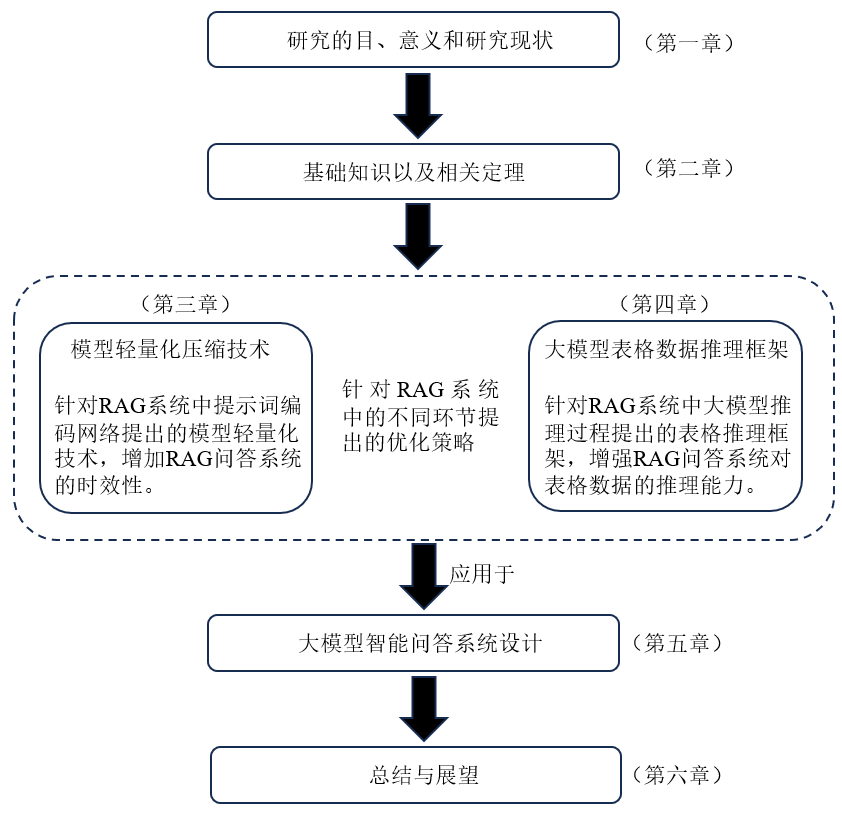
\includegraphics[scale=0.6]{章节关系.png}
  \bicaption{章节关系}{ Relationship Between Chapters}
  \label{fig:章节架构}
\end{figure}
\label{sec:first}












